\documentclass[11pt,a4paper]{book}

\usepackage{Appunti}

\begin{document}
\title{Clean Coder\\
\large{\textit{Robert C. Martin}}}
\author{Jacopo De Angelis}
\maketitle

\pagebreak
\tableofcontents
\pagebreak

\chapter{Professionalità}
\section{Prendere le proprie responsabilità}
Come si può "imparare" a prendersi le proprie responsabilità? Ci sono alcuni principi da seguire.

\section{Non fare del male}
Come può un programmatore fare del male? Può farlo al software, creando problemi per le funzioni e alla struttura del software.
\subsection{Non danneggiare la funzionalità}
Chiaramente il software deve funzionare, non solo per noi programmatori ma anche per clienti e datori di lavoro. Per essere professionali, insomma, non bisogna creare bug.
\begin{figure}[h!]
	\begin{center}
		
\includegraphics[scale=0.3]{img/001.jpg}
		\caption{Tu in questo momento}
		\label{fig: 001}
	\end{center}
\end{figure}
Il concetto è che quello deve essere l'impegno di un programmatore e nel caso escano dei bug deve prendersene la responsabilità se causati dal proprio codice.

\subsubsection{I QA non dovrebbero trovare niente}
Qual è il codice per il quale non sai se i QA\footnote{Quality assurance, coloro incaricati di testare il codice} troveranno qualcosa? Il codice di cui non si è certi.

Usare i QA come dei cacciatori di bug rende il processo più lungo e riduce la fiducia nei programmatori. Mandare in testing codice di cui non si è sicuri è violare la regola del "non fare del male".

I QA troveranno errori nel codice? Probabile.

\subsection{Devi sapere che funziona}
Come? Semplice, testando il codice.\\
Paura di metterci troppo? Automatizzali scrivendo degli unit test.\\
Quanto codice andrebbe testato? Tutto.\\
Come fare? Automatizzarli tramite suite di test.

\subsection{Non danneggiare la struttura}
In breve: devi poter fare cambiamenti senza dover ribaltare l'intera struttura.

Il problema è che in certi casi i progetti non sono estremamente flessibili e non permettono questo agio nelle modifiche. I design pattern sono qualcosa che solitamente vengono applicati pedissequamente ma una cosa da ricordare è che per una piattaforma flessibile dobbiamo essere anche noi stessi flessibili.

Quindi come fare? Quando si scopre che il codice non è così semplice da modificare allora si modifica il design per rendere più semplici i cambiamenti successivi\footnote{Belle parole se il codice non è composto da oltre 60k linee di codice}.

Un programmatore professionale cambierà il nome di un metodo o di una classe senza troppi problemi se lo riterrà necessario.\footnote{Quando si lavora in un gruppo di una certa magnitudine un cambiamento del genere rischia di essere deleterio però, è vero che gli strumenti di refactoring sono diventati più potenti ma le convenzioni di nome e di codice ci sono per un motivo.}

\subsection{Etica lavorativa}
Un programmatore è responsabile della propria educazione e del proprio miglioramento, non è un compito da affidare al datore di lavoro. Se esso aiuta con questo percorso meglio, è gentile, ma non è una sua responsabilità.

NDR: Il libro qua fa dei calcoli riguardo il tempo da dedicare al lavoro e quanto da dedicare al tempo per lo studio individuale. Non mi addentrerò in questi esempi perchè considero abbastanza sciocco fare calcoli sul tempo altrui. Propongo la lettura di \href{https://muldoon.cloud/programming/2020/04/17/programming-rules-thumb.html}{questo articolo} invece. Credo che sia più importante ricordare alle persone che non serve essere il migliore sulla piazza certe volte, magari le proprie priorità sono differenti. Non ho assolutamente nulla contro chi vuole arrivare a quei livelli, anzi, faccio loro i complimenti, ma è meglio non dimenticare che in quanto esseri umani non viviamo solo per lavorare, abbiamo anche altre passioni magari, o altri desideri. Impariamo a coltivare anche quelli. Sempre lavorare al massimo delle proprie capacità ma non per forza uccidersi dallo stress per essere i migliori in assoluto.

\subsection{Conoscere il tuo campo}
\textit{"Do you know what a Nassi-Schneiderman chart is? If not, why not? Do you
know the difference between a Mealy and a Moore state machine? You should.
Could you write a quicksort without looking it up? Do you know what the term
“Transform Analysis” means? Could you perform a functional decomposition
with Data Flow Diagrams? What does the term “Tramp Data” mean? Have you
heard the term “Conascence”? What is a Parnas Table?"}

Secondo Martin queste cose andrebbero conosciute da un programmatore. Ci terrei a precisare che probabilmente sono cose che ha imparato tramite lavoro, trovandosi davanti a nuovi problemi e nuove soluzione. Non è una colpa non conoscere qualcosa, è una colpa non voler imparare davanti ad una lacuna.

\subsection{Collaborazione}
Il secondo migliore modo per imparare è collaborare con gli altri. Un professionista si sforza per programmare in gruppo.

\subsection{Insegnamento}
Il miglior modo per imparare è farlo sapendo di doverlo spiegare ad altri.

\subsection{Conoscere il proprio dominio}
Lavori su di un programma di contabilità? Allora dovresti conoscere il campo della contabilità. Programma per agenzie di viaggi? Conoscenza dell'industria dei viaggi.

\subsection{Identificare il proprio datore di lavoro/cliente}
I problemi del tuo datore di lavoro sono i tuoi problemi. Devi dimostrare di comprendere quali essi siano e lavorare verso la loro migliore soluzione.

\subsection{Umiltà}
Per riassumere questo paragrafo: sii un buon essere umano. Sii cosciente delle tue capacità ma sentiti pronto a metterti in dubbio e fare domande. Non sapere qualcosa non è una vergogna, è normale certe volte doversi aggiornare o essere messi in questione.

Non ridicolizzare o sminuire gli altri.

\chapter{Dire di no}
\section{Ruoli avversari}
Ruoli avversari non vuol dire arrivare a puntare le lame al collo dell'altro, vuol dire che i vari attori delle discussioni hanno degli interessi lavorativi personali (far uscire il prodotto subito, sviluppare bene le funzionalità, ecc.). Un ruolo avversario positivo è quello nel quale le due parti difendono i propri interessi e cercano di trovare una soluzione nel mezzo che possa soddisfare tutti il più possibile, insomma, una soluzione pareto efficiente.

\subsection{E riguardo al perchè?}
"Fatti, non pugnette". Il perchè è meno importante del crudo fatto la maggior parte delle volte. In più spesso dare troppe spiegazioni può portare l'altro a pensare di poter gestire la cosa (e no, non in un senso da "e allora fallo tu", ma più da "quindi ora mi dici cosa fare?").

\section{Alto rischio}
Il momento migliore per dire no è quando il rischio è più alto.

\section{Sapere fare gruppo}
Un buon lavoratore in squadra comunicare frequentemente, aiutare e farsi aiutare dai colleghi, svolgere le proprie mansioni in maniera diligente. Non è colui che dice sì ogni volta.

\subsection{Provarci}
Dire "ok, ci proverò" è il peggior servizio che tu possa fare a chiunque sia coinvolto nella discussione a lavoro. "Provarci" ha vari significati in base alla parte che deve interpretare la parola; per alcuni sarà un "ce la farò", per altri un dare il contentino ma mentire spudoratamente, in certi casi si potrebbe intendere nella maniera più letterale possibile eppure si lascerebbe troppo spazio all'incertezza.

\subsection{Aggressività passiva}
Qua una delle parti più difficili: cosa fare quando ci si trova davanti ad un qualcuno che sta agendo contro gli interessi del gruppo. Si potrebbero creare prove (fondate ovviamente) che la comunicazione è sempre avvenuta in maniera trasparente in modo da parare le spalle al gruppo e permettere all'altro di fregarsi da solo o, e forse è meglio, cercare di risolvere di propria mano il problema che sta venendo creato prima del tracollo. Insomma, avvisare tutti che il treno sta arrivando e di spostarsi e filmarsi per dire di avere le prove del fatto o andare direttamente dalle persone, urlando, mettendosi a rischio, dicendo di spostarsi?

\section{Il costo di dire sì}
\href{http://raptureinvenice.com/?p=63}{Lettura consigliata nel libro}, spiega molto bene cosa voglia dire "dire sì senza pensarci" e il perchè certa gente meriti legnate sui denti.

\section{Codice impossibile}
Dopo aver letto il racconto si può evincere una cosa: dire no è importante. John avrebbe dovuto dire no alla deadline di due settimane, poi all'aggiunta di funzioni, poi al lavoro straordinario. 

Dire no è importante per noi stessi e anche per il datore di lavoro.

\chapter{Dire di sì}
\section{Il linguaggio dell'impegno}
Di'. Intendilo. Fallo.
\begin{enumerate}
	\item Tu dirai che lo farai
	\item Tu intenderai veramente ciò
	\item Tu lo farai effettivamente
\end{enumerate}

\subsection{Riconoscere la mancanza di impegno}
Secondo Martin ci sono alcune parole chiave che mostrano la mancanza di impegno:
\begin{itemize}
	\item Dovrei: "dovrei fare ciò", "dovrei perdere peso", "qualcuno dovrebbe farlo"
	\item Spero: "Spero di finire entro domani", "spero che ci incontreremo nuovamente", "spero di avere tempo per ciò"
	\item Plurale maiestatis: "incontriamoci qualche volta", "finiamo il lavoro"
\end{itemize}

\subsection{Il suono dell'impegno}
Prima pensa a cos'è effettivamente sotto il tuo controllo e poi impegnati.
\begin{figure}[h!]
	\begin{center}
		
\includegraphics[scale=0.3]{img/001.jpg}
		\caption{Tu in questo momento}
		\label{fig: 0012}
	\end{center}
\end{figure}
\footnote{Sì, nuovamente la stessa ma ehi, l'ha chiamata}.
La parola che compare più spesso quando qualcuno decide di mettere il proprio impegno in qualcosa è "io (più le sue varie declinazioni)" e poi una frase riguardante lo svolgimento di un compito. Secondo l'autore è impossibile svincolarsi da una dichiarazione d'impegno tale.
\begin{figure}[h!]
	\begin{center}
		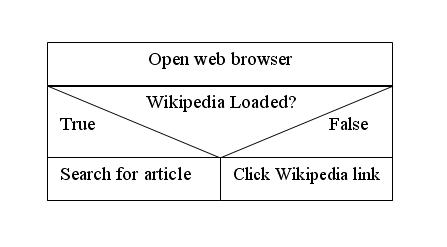
\includegraphics[scale=0.45]{img/002.jpg}
		\caption{Questa sezione è un bellissimo meme, vero?}
		\label{fig: 002}
	\end{center}
\end{figure}

Scherzi a parte, è il concetto di analizzare cosa tu sia effettivamente in grado di fare e dire che farai ciò, non cose a caso, non belle speranze.

Ecco alcune ragioni per le quali non si potrebbe intendere veramente
\subsubsection{Non funzionerebbe perchè dipendo da persona X per farlo}
Puoi fare promesse solo su ciò che controlli al 100\%.

\subsubsection{Non funzionerebbe perchè non so se possa effettivamente essere fatto}
Se non sai se X possa essere fatto, puoi dire che ti impegnerai nei passi che conducono a X.

\subsubsection{Non funzionerebbe perchè non farei in tempo}
Possono accadere cose per le quali non si può più raggiungere un certo traguardo, in quel caso è meglio avvisare subito. Se, a causa del traffico, stai arrivando in ritardo ad un appuntamento, avvisa.

\section{Imparare come dire sì}


\end{document}